% TeXiFy 似乎无法正确解析 main.tex 和 thesis-ref.bib 的关联,导致误报 UnresolvedReference
%! suppress = UnresolvedReference


\chapter{绪论}\label{ch:intro}


\section{\app 的背景与意义}\label{sec:background}

\subsection{国内外心血管疾病现状}\label{subsec:disease}

根据中国国家心血管病中心出版的《中国心血管健康与疾病报告2021》,目前中国人口心血管疾病的发病率和患病率均处于持续上升阶段,心血管疾病已成为居民死亡的首位原因;2019年,中国农村、城市心血管疾病分别占死因的46.74\%和44.26\%;心血管疾病给社会和居民带来的经济负担日益加重,且杀伤力越来越强\cite{Zhongguoxinxieguanjiankangyujibingbaogao20212022}。

不仅如此,根据世界卫生组织的统计,心血管疾病也是全球的头号死因,每年死于心血管疾病的人数多于任何其它死因;2019年,估计有1790万人死于心血管疾病,占全球死亡总数的32\%\cite{CardiovascularDiseasesCVDs}。

同时,近年来新型冠状病毒(COVID-19)的爆发也加剧了心血管疾病的危害。证据显示,既往合并心血管疾病的患者更容易在新型冠状病毒感染后发展为重症患者,死亡风险更高,预后更差\cite{zhangXinxingguanzhuangbingdufeiyanyuxinxieguanjibing2020}。

\subsection{心电监测的用途与原理}\label{subsec:monitoring}

尽早发现心血管疾病非常重要,这样就可以及时采取措施,减少疾病对患者健康的威胁\cite{CardiovascularDiseasesCVDs}。在各种心血管疾病的诊断方法中,心电图(Electrocardiogram,缩写为ECG)是最常用、最基本、最重要的一种,具有非侵入性、诊断快速、成本低廉、广泛可用等诸多优点\cite{Xinxieguanjibingzhenduanliuchengyuzhiliaocelue2007}。

心电图是对心电信号的记录。通过放置在皮肤上的电极可以检测到心脏的电活动,将电压与时间的关系绘制为二维图像就得到了心电图,如图\ref{fig:10sec-ekg-lead}所示。

\begin{figure}
    \centering
    % 这个大小刚好可以把 \subsection{静态与动态心电图} 挤到下一页,但不会把自己挤下去
    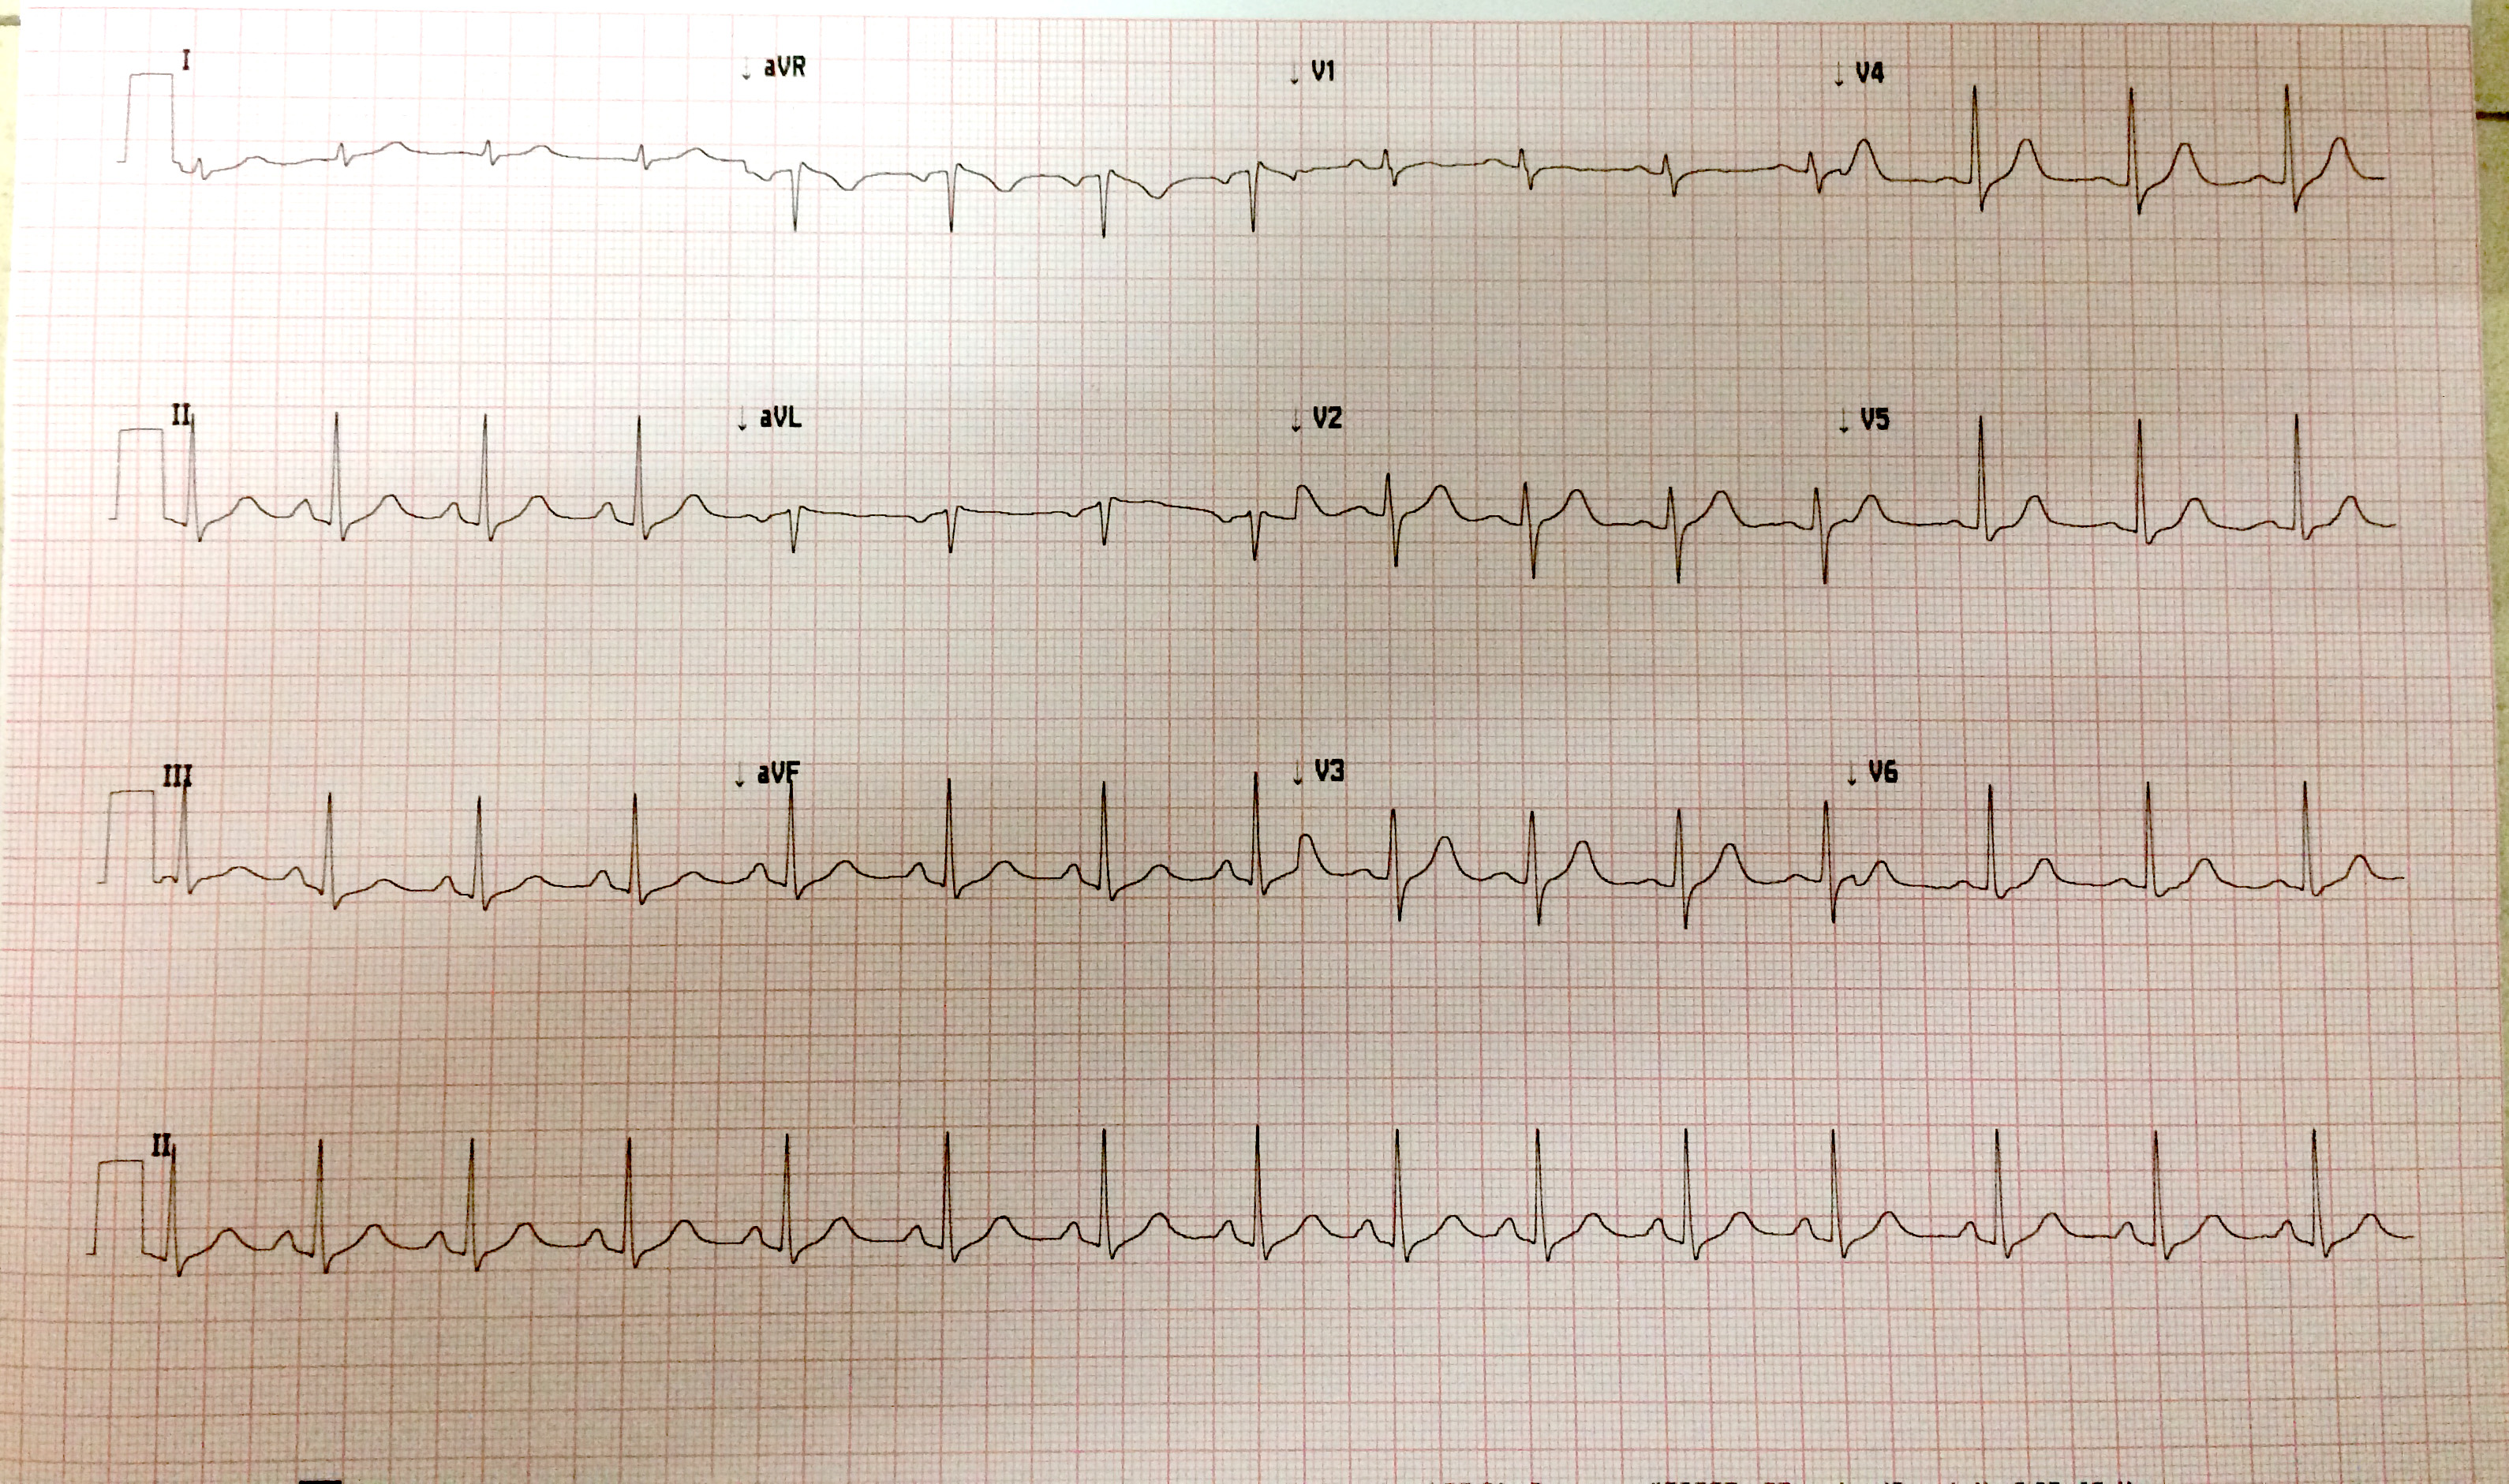
\includegraphics[width=.63\textwidth]{../assets/10sec-ekg-lead}
    \bicaption{一张10秒12导联心电图}{A 10-second 12-lead ECG}\label{fig:10sec-ekg-lead}
\end{figure}

\subsection{常规心电图与动态心电图}\label{subsec:standard-holter}

心电图有两种主要类型:常规心电图(Standard ECG)和动态心电图(Holter ECG、Dynamic ECG或Ambulatory ECG)。

常规心电图,也被称为静息心电图(Resting ECG),是在患者保持静止状态时记录的心电图。常规心电图的记录需要在专业的医疗机构中进行,患者通常处于平躺状态,在四肢和胸部表面安装电极,电极检测心脏产生的电信号并将其传输到心电图仪器。常规心电图通常包含12个导联\footnote{这里的一个导联是指一对电极之间的电势差,比如Ⅱ导联是指右臂电极和腿电极之间的电势差。另外,连接电极与心电图仪器的电缆也常被称为导联。本文中无特别说明的情况下,导联均指电势差而非电缆。},一次记录10秒,并打印在心电图纸\footnote{心电图纸包含红色的坐标线,每1mm一小格(用细线分隔),每5mm一大格(用粗线分隔)。横轴一小格表示40ms,一大格表示200ms。纵轴一小格表示0.1mV,一大格表示0.5mV。}上。图\ref{fig:10sec-ekg-lead}就是一张常规心电图。

动态心电图则是在患者进行日常生活活动时记录的心电图。动态心电图的记录可以在几乎任何环境进行,只需要患者佩戴动态心电记录仪(Holter monitor)即可。动态心电记录仪是一种便携式可穿戴设备,可在较长时间内(24小时以上)记录心脏的电活动,有助于检出非持续性心律失常。统计显示,动态心电图在临床诊断中对心肌缺血及各种心律失常事件的检出率都明显高于常规心电图\cite{zhengDongtaixindiantuyuchangguixindiantuzhenduanguanxinbinghuanzhexinjiquexiejixinlushichangdelinchuangxiaoguobijiao2011}。

\subsection{心电自动诊断技术}\label{subsec:diagnosis}

\todo{心电自动诊断技术的必要性,动态心电图数据量太大}

基于可穿戴设备对心电数据进行实时分析可以及时发现患者的异常状况,为患者提供随时随地的医疗监护,降低心血管疾病对患者健康的威胁。

\subsubsection{心电分割算法}\label{subsubsec:segmentation}

\todo{todo}

\subsubsection{心电分类算法}\label{subsubsec:classification}

\todo{todo}

\subsubsection{移动端心电自动诊断}\label{subsubsec:mobile}

\todo{todo}


\section{国内外\app 现状}\label{sec:status}

\todo{相关研究领域的现状和研究进展分析,或与应用系统研发相关的技术发展现状}

当前国内外已有不少基于可穿戴设备的远程心电监测系统,其中一些使用了手动编写的算法\cite{zhengJiyukechuandaishebeideyidongjianhuAPP2019,wuYidongxindianjiancexitongdeyanjiuyushixian2018,chenYidongxindianxinxijianhuxitongjixindianjiancesuanfadeyanjiu2018,heJiyuyidongpingtaidexindianjianceyiliaoxitongdeshixian2017,gradlRealtimeECGMonitoring2012,wenRealtimeECGTelemonitoring2008},另一些则使用了机器学习技术。使用机器学习技术的系统大致可以分为两类:一类是在移动端只对数据进行简单统计,完整的算法模型则部署于服务端\cite{wangJiyushenduxuexideyidongyuanchengxindianjiancexitongshejiyushixian2020,singhSmartECGMonitoring2022}。患者如果想获取完整的分析报告,则需要将数据上传至服务端后,等待服务端分析完成。在这类系统中,患者能在移动端立即获取的结果较少,而完整分析结果可能因为网络质量差、服务端算力不足等原因而有较大延迟。另一类则是边缘计算架构,将模型部署在移动端,数据分析直接在移动端进行\cite{chenJiyushenduxuexidexindianfenximoxingdeshejiyuyouhua2021,liuJiyuyidongzhongduanfenxidekechuandairouxingxindianjiancexitong2021,wangEnablingSmartPersonalized2014,jinPredictingCardiovascularDisease2009}。这样可以缩短延迟,节省带宽,并节省了高算力服务器的成本。但已有的少数此类应用都只实现了极简单的功能,旨在以演示程序验证模型正确性,并没有进行完整的应用开发。此外,此类演示程序均只进行了Android平台的开发。


\section{本项目的主要工作}\label{sec:work}

\todo{
    本选题与现有研究工作或应用系统之间的区别。
    本选题的主要研究内容、重点和特点,着重论述学生本人将完成的工作。
    论文预期达到的目标,包括提出的新方法或新技术、对现有技术的改进、或所研发系统的功能等内容。
}

本选题与上述最后一类系统相似,与已有应用系统的主要区别在于两点:其一是包含较完整的产品功能,可以投入到实际使用中;其二是基于跨平台开发框架,同时支持Android平台和iOS平台的移动设备。课题的选题来源于导师心电图课题的子项目,该课题目前已基于PyTorch训练了心电数据分类模型,并使用Python编写了相关算法,下一阶段的目标是将模型部署至移动端,课题目标明确,并已经具备较好的人工智能算法模型的技术支撑。


\section{论文组织结构}\label{sec:structure}

\todo{todo}
